\documentclass[conference]{IEEEtran}
\usepackage{cite}
\usepackage{amsmath,amssymb,amsfonts}
\usepackage{graphicx}
\usepackage{xcolor}
\usepackage[hidelinks]{hyperref}
\def\BibTeX{{\rm B\kern-.05em{\sc i\kern-.025em b}\kern-.08em
    T\kern-.1667em\lower.7ex\hbox{E}\kern-.125emX}}
\begin{document}

\title{Mitigating Physical Layer Vulnerabilities in 6G Communications using Deep Reinforcement Learning}

\author{\IEEEauthorblockN{Abd Alsalam HIJAZI KELANI}
\IEEEauthorblockA{\textit{Dept. of Computer Engineering} \\
\textit{Biruni University}\\
Istanbul, Turkey \\
251132908@st.biruni.edu.tr}
\and
\IEEEauthorblockN{Ghaith ALMADANI}
\IEEEauthorblockA{\textit{Dept. of Computer Engineering} \\
\textit{Biruni University}\\
Istanbul, Turkey \\
251132902@st.biruni.edu.tr}
\and
\IEEEauthorblockN{Dr. Mhd Raja ABOU HARB}
\IEEEauthorblockA{\textit{Dept. of Computer Engineering} \\
\textit{Biruni University}\\
Istanbul, Turkey \\
mharb@biruni.edu.tr}
}


\maketitle

\begin{abstract}
Sixth-generation (6G) wireless communication systems are expected to support ultra-high data rates, ultra-low latency, and massive connectivity. However, the dynamic nature of wireless communication introduces major physical layer security challenges, including jamming and eavesdropping attacks.
This paper proposes a Deep Reinforcement Learning (DRL)-based adaptive security framework using the Deep Q-Network (DQN) algorithm to mitigate physical layer vulnerabilities in 6G communication systems. The proposed framework dynamically optimizes transmission parameters such as beamforming direction, transmit power allocation, and artificial noise injection to maximize secrecy rate and reduce the impact of adversarial attacks in real time.
The wireless environment is modeled as a Markov Decision Process (MDP), where the DQN agent learns optimal security strategies through continuous interaction with the environment. In addition, a lightweight simulation-based evaluation is conducted to compare the adaptive DRL-based strategy against two non-adaptive baselines: a static random policy and a threshold-based heuristic policy derived from domain knowledge. The proposed work contributes toward the development of intelligent and adaptive physical layer security solutions for future 6G networks.
\end{abstract}
\begin{IEEEkeywords}
6G Communications, Physical Layer Security, Deep Reinforcement Learning (DRL), Deep Q-Network (DQN), Beamforming, Anti-Jamming, Eavesdropping, Wireless Security, Artificial Intelligence, Secrecy Rate
\end{IEEEkeywords}
\section{Introduction}

Sixth-generation (6G) wireless communication systems are expected to support ultra-high data rates, ultra-low latency, massive connectivity, and intelligent networking applications. Emerging technologies such as Terahertz (THz) communication, massive multiple-input multiple-output (MIMO), and artificial intelligence-driven networking are anticipated to play a major role in future communication infrastructures. These technologies are expected to support advanced applications including autonomous vehicles, smart cities, industrial automation, and large-scale Internet of Things (IoT) environments \cite{b1,b6}.

Despite these advancements, the security of wireless communication systems remains a major challenge. Due to the broadcast nature of wireless propagation, wireless communication systems are inherently vulnerable to interception, interference, and unauthorized access. Consequently, 6G networks face significant physical layer security threats, including jamming, spoofing, and eavesdropping attacks by malicious entities \cite{b1,b4,b6}. In dynamic wireless environments, attackers may continuously adapt their behavior, making conventional static security mechanisms insufficient for maintaining secure communication.

Traditional wireless security approaches mainly rely on cryptographic techniques implemented at higher communication layers. Although these methods provide strong protection for data confidentiality, they may introduce computational overhead, latency, and scalability limitations in large-scale 6G environments. Furthermore, conventional cryptographic methods alone cannot fully protect the wireless transmission medium from physical layer attacks such as signal interference and unauthorized interception \cite{b6}.

To address these challenges, Physical Layer Security (PLS) has emerged as a promising complementary security approach that exploits wireless channel characteristics to improve communication confidentiality and robustness. In addition, recent advancements in Artificial Intelligence (AI) and Deep Reinforcement Learning (DRL) have introduced new opportunities for adaptive wireless security optimization. DRL enables intelligent agents to learn optimal decision-making strategies through continuous interaction with the environment, making it highly suitable for dynamic and adversarial 6G scenarios \cite{b2,b3,b4,b5}.

Several recent studies have investigated the integration of DRL and PLS in wireless communication systems. Mahmoud et al. \cite{b1} proposed a deep learning-based physical layer security framework capable of detecting spoofing, jamming, and eavesdropping attacks in 6G networks. Kamal et al. \cite{b2} explored DRL-assisted STAR-RIS optimization for improving secrecy performance in secure multi-user communication systems. Similarly, Lin et al. \cite{b3} introduced a GAN-powered DRL framework for enhancing physical layer security in cognitive IoT environments. Lu et al. \cite{b4} presented a comprehensive survey on reinforcement learning-based physical and cross-layer security techniques for future 6G networks. Belgacem and Belgacem \cite{b5} investigated reinforcement learning-based RIS optimization for covert 6G communication systems, while Mitev et al. \cite{b6} discussed the role of physical layer security as a complementary security mechanism for future wireless networks.

Although existing studies demonstrate the potential of DRL and PLS techniques for securing wireless systems, many approaches focus on isolated attack scenarios or static optimization strategies. In highly dynamic 6G environments, there is still a need for adaptive and intelligent frameworks capable of mitigating multiple physical layer attacks in real time.

In this paper, we propose a Deep Reinforcement Learning (DRL)-based adaptive security framework using the Deep Q-Network (DQN) algorithm to mitigate physical layer vulnerabilities in 6G communication systems. The proposed framework dynamically adjusts transmission parameters such as beamforming direction, transmit power allocation, and artificial noise injection to improve secrecy performance and reduce the impact of jamming and eavesdropping attacks.

The main contributions of this work are summarized as follows:

\begin{itemize}

\item Proposing a DQN-based adaptive framework for enhancing physical layer security in 6G communication systems.

\item Modeling dynamic attack scenarios including jamming and eavesdropping attacks.

\item Enhancing communication secrecy using adaptive beamforming, transmit power optimization, and artificial noise injection.

\item Providing a lightweight prototype evaluation comparing the adaptive DRL-based strategy against a static random baseline and a threshold-based heuristic policy, demonstrating consistent superiority of the learned approach.

\end{itemize}

The remainder of this paper is organized as follows. Section II reviews related work on physical layer security and reinforcement learning for wireless communication systems. Section III presents the proposed system model and DRL-based framework. Section IV discusses the experimental evaluation and results. Finally, Section V concludes the paper and discusses future research directions.


\section{Related Work}

Physical Layer Security (PLS) has emerged as a promising solution for securing next-generation wireless communication systems. Unlike traditional cryptographic methods that mainly operate at higher layers of the communication stack, PLS exploits the characteristics of wireless propagation channels such as fading, interference, noise, and spatial diversity to enhance communication confidentiality and robustness. Mitev et al. \cite{b6} discussed the importance of PLS in future 6G networks and highlighted its ability to complement conventional cryptographic approaches by supporting secure key generation, authentication, and protection against jamming and eavesdropping attacks.

Recent advancements in Artificial Intelligence (AI) and Deep Learning (DL) have introduced new opportunities for improving physical layer security in highly dynamic wireless environments. Mahmoud et al. \cite{b1} proposed an advanced security framework for 6G networks that integrates deep learning techniques with physical layer security mechanisms. Their framework utilized deep neural networks and hybrid learning models to detect spoofing, jamming, and eavesdropping attacks. The study demonstrated significant improvements in attack detection accuracy and communication robustness under adversarial conditions. However, the proposed framework mainly focuses on attack detection rather than adaptive real-time mitigation.

Reinforcement Learning (RL) has also gained significant attention as an intelligent optimization approach for wireless security. Lu et al. \cite{b4} presented a comprehensive survey on reinforcement learning-based physical and cross-layer security in 6G communication systems. Their work reviewed various RL applications for mitigating jamming, spoofing, eavesdropping, and privacy leakage attacks. The survey emphasized that RL-based techniques are particularly suitable for dynamic wireless environments because they can continuously learn optimal security strategies without requiring complete prior knowledge of attack models. Nevertheless, challenges such as training instability, computational complexity, and partial channel observation remain open research problems.

Deep Reinforcement Learning (DRL) has recently been applied to optimize secure communication in intelligent wireless systems. Kamal et al. \cite{b2} proposed a DRL-assisted STAR-RIS framework for secure multi-user Integrated Sensing and Communication (ISAC) systems in 6G networks. Their work jointly optimized beamforming vectors, STAR-RIS coefficients, and receive filters to maximize secrecy rate in the presence of multiple eavesdroppers. The study demonstrated the effectiveness of DRL in solving complex non-convex optimization problems associated with secure communication systems.

Similarly, Lin et al. \cite{b3} introduced a GAN-powered DRL framework for enhancing physical layer security in energy-harvesting cognitive Internet of Things (IoT) networks. Their approach jointly optimized transmission power allocation and energy harvesting duration to improve secrecy rate while reducing secrecy outage probability. This work highlighted the ability of DRL to simultaneously address both security and energy efficiency requirements in future wireless systems.

Covert communication techniques have also been explored to further improve physical layer security in future 6G architectures. Belgacem and Belgacem \cite{b5} proposed a reinforcement learning-based relay and Reconfigurable Intelligent Surface (RIS) optimization framework for covert 6G ground station communications. Their approach optimized relay trajectories, RIS phase shifts, and transmission power allocation while minimizing the probability of detection by adversarial entities. The study demonstrated the capability of reinforcement learning to support adaptive and low-probability-of-detection communication in highly dynamic wireless environments.

Although existing studies demonstrate the effectiveness of PLS, DRL, RIS, and AI-based optimization techniques for securing wireless systems, many current approaches focus on isolated attack scenarios or specific optimization objectives. Some methods primarily address attack detection, while others focus on secrecy rate optimization or covert communication individually. Therefore, there remains a need for a unified adaptive framework capable of dynamically mitigating multiple physical layer attacks, including jamming and eavesdropping, in real-time 6G communication environments. In contrast to RIS-assisted works reviewed above, the proposed prototype in this paper focuses on a simplified non-RIS scenario based on adaptive power allocation, beamforming control, and artificial noise injection. This limitation keeps the experimental scope practical while preserving the main objective of adaptive physical layer security.


\section{System Model and Methodology}

This section presents the proposed Deep Reinforcement Learning (DRL)-based adaptive framework for mitigating physical layer vulnerabilities in future 6G communication systems. The proposed framework focuses on dynamically protecting wireless communication channels against jamming and eavesdropping attacks through intelligent optimization of transmission parameters.

\subsection{System Model}

The considered wireless communication environment consists of a legitimate Base Station (BS), a legitimate mobile user, and one or more malicious adversaries attempting to intercept or disrupt communication. The adversarial entities may operate either as eavesdroppers or jammers within the wireless environment.

The Base Station communicates with the legitimate user using highly directional beamforming techniques. Meanwhile, malicious entities continuously attempt to degrade communication quality or intercept confidential transmissions. Due to the dynamic nature of future 6G communication environments, channel conditions, user mobility, and attacker behavior may continuously change over time.

To address these challenges, the proposed framework integrates a Deep Reinforcement Learning agent capable of observing the wireless environment and dynamically adapting transmission strategies in real time. The DRL agent continuously monitors wireless channel characteristics and optimizes transmission parameters to maximize secrecy performance and communication robustness.

\subsection{Threat Model}

The proposed framework considers two major physical layer attacks commonly expected in future 6G communication systems:

\begin{itemize}

\item \textbf{Jamming Attacks:} In this attack scenario, the adversary intentionally transmits interference signals to degrade the quality of the legitimate communication channel and reduce communication reliability.

\item \textbf{Eavesdropping Attacks:} In this scenario, a malicious entity attempts to intercept confidential wireless transmissions without authorization in order to extract sensitive information.

\end{itemize}

The attacker is assumed to be mobile and adaptive, meaning that attack patterns and wireless channel conditions may dynamically change during communication sessions. This assumption reflects the highly dynamic and intelligent nature of future 6G wireless environments.

\subsection{Deep Reinforcement Learning Framework}

The proposed framework utilizes the Deep Q-Network (DQN) algorithm as the core Deep Reinforcement Learning technique. The wireless communication environment is modeled as a Markov Decision Process (MDP), where the DQN agent continuously interacts with the environment to learn optimal security strategies.

At each time step, the DRL agent observes the current wireless environment state, selects an appropriate transmission action, receives a reward value based on communication performance, and updates its policy accordingly. Through continuous interaction with the environment, the DQN agent gradually learns adaptive strategies that improve communication secrecy and reduce the effectiveness of adversarial attacks.

The DRL agent dynamically optimizes several transmission parameters, including:

\begin{itemize}

\item Transmit power allocation

\item Beamforming direction optimization

\item Artificial noise injection

\end{itemize}

The adaptive optimization process enables the communication system to intelligently respond to changing wireless conditions and adversarial behavior in real time.

Figure~\ref{fig:drl_framework} illustrates the overall workflow of the proposed DQN-based adaptive physical layer security framework. The DQN agent continuously interacts with the wireless environment, dynamically optimizes transmission actions, and updates its policy based on secrecy-oriented reward feedback.

\begin{figure}[htbp]
\centering
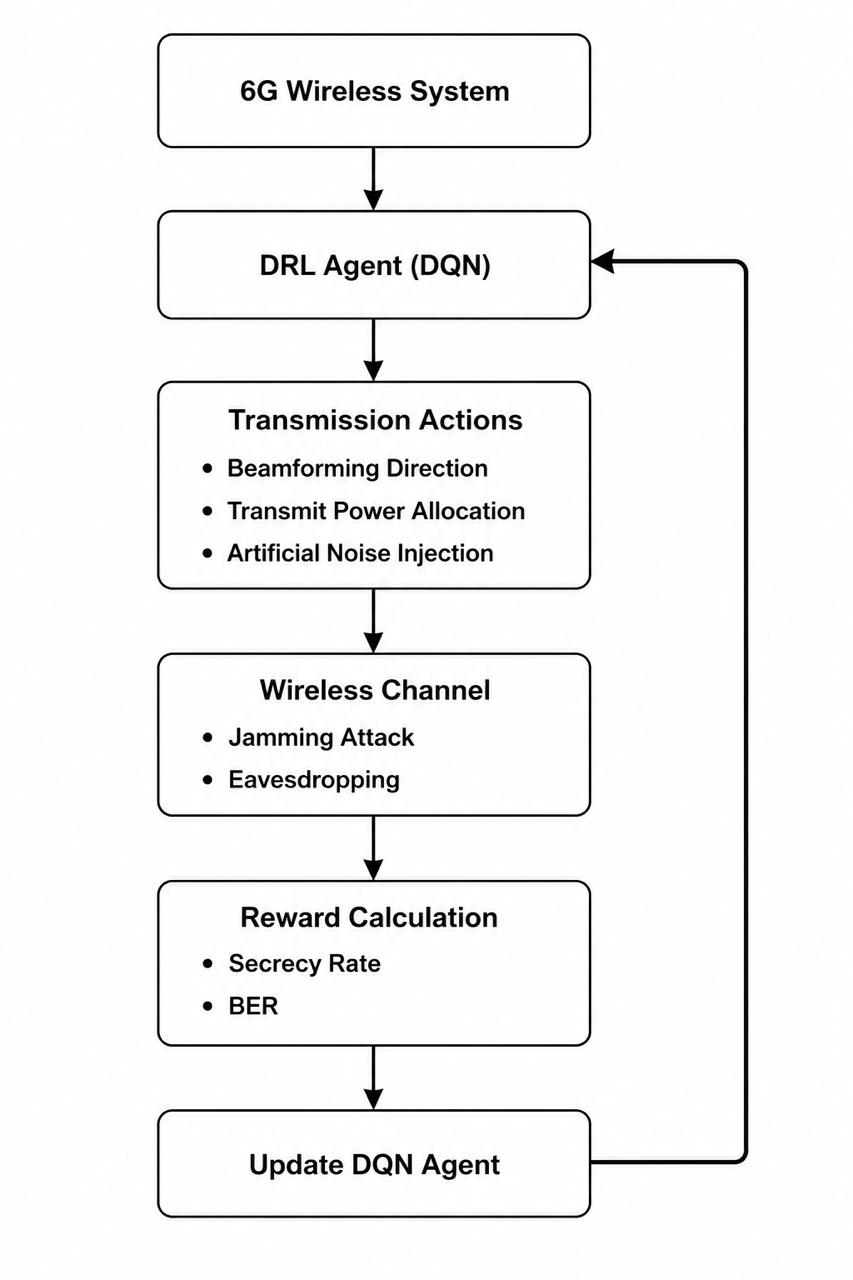
\includegraphics[width=0.8\columnwidth]{2026-05-20 22.19.28.jpg}
\caption{Proposed DRL-based adaptive physical layer security framework for 6G communication systems.}
\label{fig:drl_framework}
\end{figure}

\subsection{Markov Decision Process Formulation}

The wireless security optimization problem is formulated as a Markov Decision Process consisting of states, actions, and rewards.

The state space is represented as:

\begin{equation}
S_t = \{CSI,\ SINR,\ P_j,\ d_e\}
\end{equation}

where \(CSI\) represents channel state information, \(SINR\) denotes the signal-to-interference-plus-noise ratio, \(P_j\) represents jammer power, and \(d_e\) denotes the normalized distance between the eavesdropper and the legitimate user.

The action space of the DQN agent is defined as:

\begin{equation}
A_t = \{P_t, w_t, N_t\}
\end{equation}

where \(P_t\) represents transmission power allocation, \(w_t\) denotes beamforming control, and \(N_t\) represents artificial noise injection level.

The secrecy rate is defined as:

\begin{equation}
R_s = [C_b - C_e]^+
\end{equation}

where \(C_b\) represents the legitimate channel capacity and \(C_e\) represents the eavesdropper channel capacity.

The reward function utilized for DQN training is defined as:

\begin{equation}
R_t = \alpha R_s - \beta E - \gamma BER
\end{equation}

where \(R_s\) denotes the secrecy rate, \(E\) represents energy consumption, \(BER\) denotes bit error rate, and \(\alpha\), \(\beta\), and \(\gamma\) are weighting parameters used to balance security and communication performance objectives. In the prototype implementation, these are set to \(\alpha = 5\), \(\beta = 1\), and \(\gamma = 0.5\), prioritizing secrecy rate maximization while penalizing jammer interference and noise-induced degradation.

\subsection{State Space Vectorization}

In the prototype implementation, the state vector is represented as a normalized four-dimensional float32 array $\mathbf{S}_t = [s,\, p_j,\, n,\, d_e]^{\top}$, where $s \in [0,1]$ denotes normalized signal strength (serving as a proxy for channel state information, CSI), $p_j \in [0,1]$ represents normalized jammer interference power, $n \in [0,1]$ denotes normalized noise level (from which SINR can be approximated as $s/(n + \epsilon)$), and $d_e \in [0,1]$ represents the normalized distance between the eavesdropper and the legitimate user. All four variables are uniformly initialized in $[0,1]$ at the start of each episode and hard-clipped to this range at every simulation step to ensure bounded observations. The resulting 4D vector is directly passed as the flattened observation input to the MLP policy network without further preprocessing.

The secrecy rate in the prototype is computed at each step as:
\begin{equation}
R_s = s - (1 - d_e) = s + d_e - 1
\end{equation}
which increases when signal strength is high and the eavesdropper is far from the legitimate user, consistent with standard physical layer security formulations where $C_b > C_e$ implies positive secrecy capacity.

\subsection{Prototype Evaluation Strategy}

To evaluate the proposed framework, a lightweight simulation-based prototype environment is considered. The DQN agent is trained through iterative interaction with a simulated wireless environment comprising legitimate communication users and adversarial entities.

The evaluation compares the adaptive DRL-based strategy against two non-adaptive baselines: (1) a static random policy that uniformly samples from the action space, and (2) a Threshold-Based Heuristic Policy (TBHP) that applies domain-knowledge rules without any learning capability. The TBHP increases transmit power when signal strength falls below 0.6, injects artificial noise when eavesdropper distance falls below 0.7, and applies beam adjustment otherwise. Key evaluation metrics include average reward, secrecy rate, communication robustness, and resistance against jamming and eavesdropping attacks.

The proposed framework aims to demonstrate the potential of Deep Reinforcement Learning for enabling intelligent and adaptive physical layer security mechanisms in future 6G communication systems.

\section{Experimental Evaluation and Discussion}

The proposed Deep Q-Network (DQN)-based physical layer security framework was evaluated in a simulated 6G wireless communication environment under dynamic jamming and eavesdropping conditions. The DQN agent was trained through continuous interaction with the environment and compared against two non-adaptive baselines: (1) a static random policy that uniformly samples from the action space at each step, and (2) a Threshold-Based Heuristic Policy (TBHP) that encodes domain knowledge about physical layer security through fixed decision rules, without any learning capability.

The simulation environment was implemented in Python using a lightweight custom wireless communication model. Dynamic wireless conditions were simulated by varying channel quality, jammer interference power, and eavesdropping behavior during training episodes. The DQN agent continuously interacted with the environment to learn adaptive transmission strategies under changing attack scenarios.

The DQN agent utilized a multilayer perceptron (MLP) neural network architecture consisting of two hidden layers with ReLU activation functions, trained using the Adam optimizer with a learning rate of $1\times10^{-3}$ and a discount factor of $\gamma = 0.99$. An epsilon-greedy exploration strategy was applied to balance exploration and exploitation during training. An experience replay buffer of 10,000 samples with a mini-batch size of 32 was employed to improve training stability. The training process was conducted over 5,000 simulation timesteps in a dynamic wireless environment involving varying jammer interference and eavesdropping conditions. Table~\ref{tab:sim_params} provides the complete set of simulation and training parameters for reproducibility.

\begin{table}[htbp]
\caption{Simulation Environment and Training Hyperparameters}
\centering
\begin{tabular}{|l|c|}
\hline
\textbf{Parameter} & \textbf{Value} \\
\hline
State space dimensionality & 4 \\
State variable range & {[}0,\,1{]} (normalized) \\
Action space & 5 discrete actions \\
BS--User distance (normalized) & 1.0 (fixed) \\
Initial eavesdropper distance & $\mathcal{U}(0,1)$ \\
Initial jammer power & $\mathcal{U}(0,1)$ \\
Jammer power drift per step & $\pm 0.03$ \\
Noise level drift per step & $\pm 0.02$ \\
Jammer effect on signal & $-0.05 \times p_j$ per step \\
MLP hidden layers & $2 \times 64$ neurons \\
Activation function & ReLU \\
Optimizer & Adam \\
Learning rate & $1\times10^{-3}$ \\
Discount factor ($\gamma$) & 0.99 \\
Replay buffer size & 10,000 \\
Mini-batch size & 32 \\
Exploration & $\varepsilon$-greedy ($\varepsilon$: $1.0\!\to\!0.05$) \\
Total training timesteps & 5,000 \\
Independent evaluation runs & 10 \\
\hline
\end{tabular}
\label{tab:sim_params}
\end{table}

\begin{table}[htbp]
\caption{Performance Comparison: DQN, Static Random, and Threshold-Based Heuristic Policy (TBHP)}
\centering
\resizebox{\columnwidth}{!}{

\begin{tabular}{|c|c|c|c|c|c|}
\hline
\textbf{Run} & \textbf{DQN Reward} & \textbf{Static Random} & \textbf{TBHP Reward} & \textbf{DQN vs.\ Static (\%)} & \textbf{DQN vs.\ TBHP (\%)} \\
\hline
1  & 4.281603 & 2.737537 & 2.980000 & $+56.40$ & $+43.68$ \\
2  & 3.710249 & 2.406413 & 2.710000 & $+54.18$ & $+36.91$ \\
3  & 4.245277 & 2.575250 & 2.950000 & $+64.85$ & $+43.91$ \\
4  & 1.516637 & 2.472241 & 2.430000 & $-38.65$ & $-37.59$ \\
5  & 3.905068 & 2.634122 & 2.840000 & $+48.23$ & $+37.50$ \\
6  & 4.254050 & 2.666850 & 2.960000 & $+59.52$ & $+43.72$ \\
7  & 4.177467 & 2.422829 & 2.870000 & $+72.42$ & $+45.56$ \\
8  & 4.303623 & 2.596722 & 2.920000 & $+65.73$ & $+47.38$ \\
9  & 4.228331 & 2.575458 & 2.830000 & $+64.18$ & $+49.41$ \\
10 & 3.800821 & 2.605198 & 2.800000 & $+45.89$ & $+35.74$ \\
\hline
\textbf{Avg.} & \textbf{3.842913} & \textbf{2.569262} & \textbf{2.829000} & $\mathbf{+49.28}$ & $\mathbf{+35.84}$ \\
\hline
\end{tabular}

}

\label{tab:dqn_results}
\end{table}
Table~\ref{tab:dqn_results} summarizes the performance comparison among the adaptive DQN-based framework, the static random baseline, and the Threshold-Based Heuristic Policy (TBHP) across ten independent simulation runs. The results demonstrate that the proposed DRL-based approach consistently achieved higher reward values than both baselines in most experimental scenarios.
As shown in Fig.~\ref{fig:reward_comparison}, the proposed DQN-based framework achieved higher average reward values than both baselines in most simulation runs.

\begin{figure}[htbp]
\centering
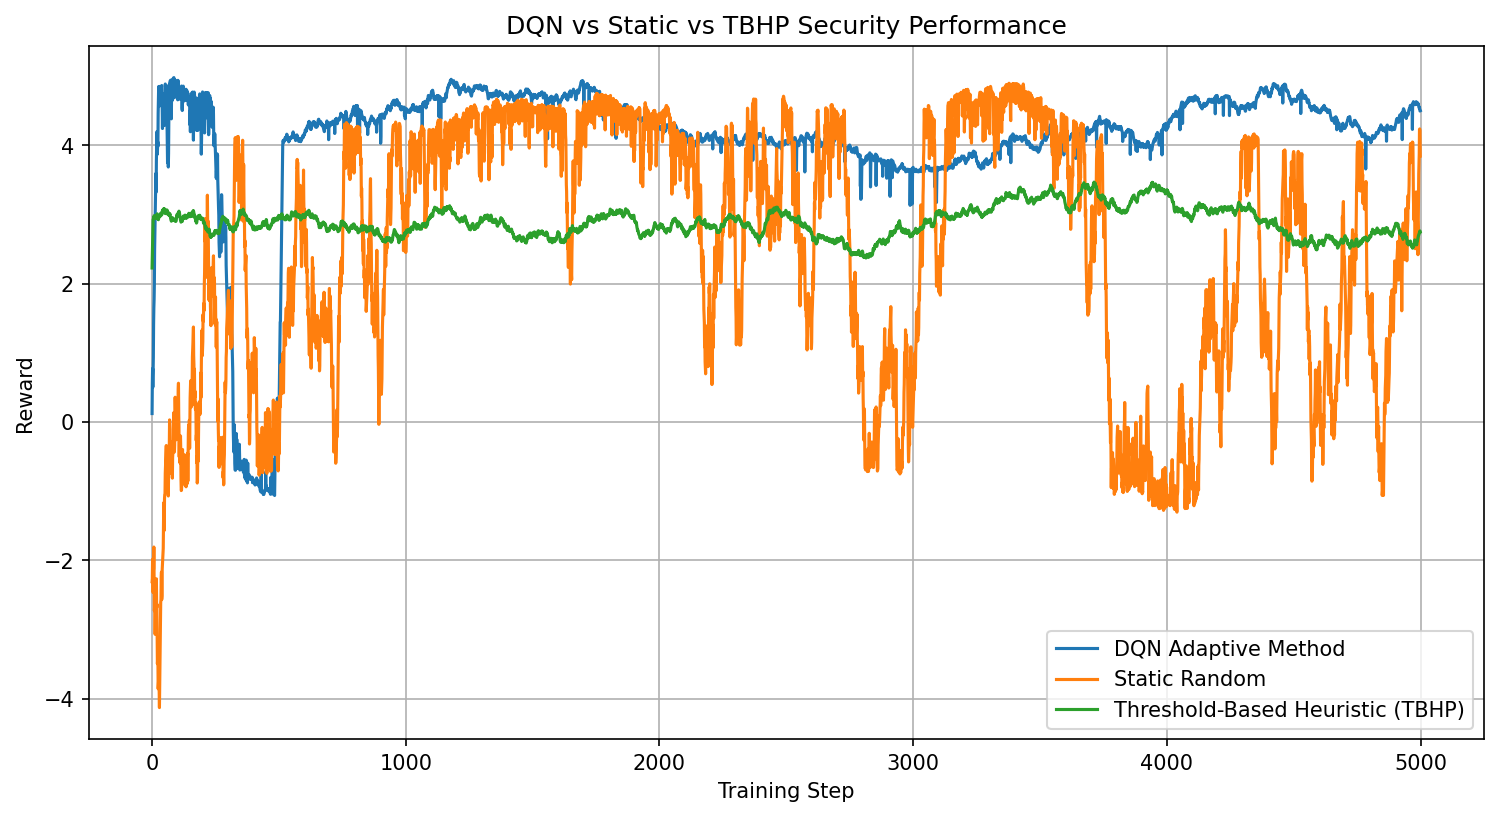
\includegraphics[width=\columnwidth]{graph.png}
\caption{Average reward comparison among the proposed DQN-based framework, the static random baseline, and the Threshold-Based Heuristic Policy (TBHP) across 10 independent simulation runs.}
\label{fig:reward_comparison}
\end{figure}

The DQN-based framework achieved an average reward of 3.842913, compared to 2.569262 for the static random baseline and 2.829000 for the TBHP. Overall, the DQN achieved an average improvement of approximately 49.28\% over the static random baseline and approximately 35.84\% over the domain-knowledge-based TBHP, demonstrating that adaptive learned strategies outperform both uninformed random selection and manually-engineered deterministic rules.


The reward convergence behavior indicated that the DQN agent successfully learned adaptive transmission strategies capable of mitigating the effects of jamming and eavesdropping attacks. In most simulation runs, the adaptive framework maintained higher secrecy-oriented reward values due to its ability to dynamically optimize beamforming direction, transmission power allocation, and artificial noise injection.


Although one experimental run (Run 4) produced lower performance than both baselines, the overall results demonstrate that reinforcement learning techniques can significantly improve physical layer security in dynamic wireless environments. Notably, the TBHP also outperformed the DQN in Run 4, further confirming that this particular run represents an outlier rather than a systematic weakness. The observed fluctuations are primarily attributed to random initial environment states, stochastic jammer behavior, and exploration-driven decisions during early training.
In particular, Run 4 produced lower performance due to unfavorable initial conditions combined with aggressive epsilon-greedy exploration, which temporarily degraded learning stability. This result highlights the sensitivity of reinforcement learning to highly adversarial initial states and motivates future work on more robust warm-start training strategies.

In addition, secrecy rate tracking results showed that the DQN agent maintained more stable secrecy performance during communication sessions. These findings highlight the potential of Deep Reinforcement Learning for enabling intelligent and adaptive security mechanisms in future 6G communication systems.

\subsection{Limitations}

The current prototype is based on a simplified wireless simulation environment and does not fully represent real-world 6G communication complexity. In addition, the proposed framework was evaluated using a single-agent DQN architecture under limited attack scenarios. Future work may extend the framework using more realistic wireless channel models, multi-agent reinforcement learning, and large-scale 6G network simulations.

\section{Conclusion}

This paper presented a Deep Reinforcement Learning-based physical layer security framework for future 6G wireless communication systems. The proposed framework utilized the Deep Q-Network (DQN) algorithm to dynamically optimize transmission strategies in the presence of jamming and eavesdropping attacks.

The wireless communication environment was modeled as a Markov Decision Process (MDP), enabling the DQN agent to continuously learn adaptive security strategies through interaction with the environment. The proposed framework dynamically adjusted beamforming direction, transmission power allocation, and artificial noise injection to improve secrecy performance and communication robustness.

Experimental evaluation results demonstrated that the proposed adaptive framework consistently outperformed both non-adaptive baselines. Across ten simulation runs, the DQN-based framework achieved an average performance improvement of approximately 49.28\% over the static random baseline and approximately 35.84\% over the domain-knowledge-based threshold heuristic, while maintaining stable secrecy-oriented communication performance under dynamic wireless conditions.

The obtained results indicate that Deep Reinforcement Learning can play an important role in developing intelligent and autonomous physical layer security mechanisms for future 6G communication systems. Future work may extend the proposed framework by integrating more advanced DRL algorithms, multi-agent communication scenarios, and large-scale realistic 6G network environments.

\begin{thebibliography}{00}

\bibitem{b1} H. Mahmoud, T. Ismail, T. Baiyekusi, and M. Idrissi, ``Advanced security framework for 6G networks: Integrating deep learning and physical layer security,'' \textit{Network}, vol. 4, pp. 453--467, 2024, doi: 10.3390/network4040023.

\bibitem{b2} M. M. Kamal, S. Z. U. Abideen, M. A. Al-Khasawneh, A. Alabrah, R. S. A. Larik, and M. I. Marwat, ``Optimizing secure multi-user ISAC systems with STAR-RIS: A deep reinforcement learning approach for 6G networks,'' \textit{IEEE Access}, 2025, doi: 10.1109/ACCESS.2025.3542607.

\bibitem{b3} R. Lin, H. Qiu, J. Wang, Z. Zhang, L. Wu, and F. Shu, ``Physical-layer security enhancement in energy-harvesting-based cognitive Internet of Things: A GAN-powered deep reinforcement learning approach,'' \textit{IEEE Internet of Things Journal}, vol. 11, no. 3, pp. 4899--4913, Feb. 2024.

\bibitem{b4} X. Lu, L. Xiao, P. Li, X. Ji, C. Xu, S. Yu, and W. Zhuang, ``Reinforcement learning-based physical cross-layer security and privacy in 6G,'' \textit{IEEE Communications Surveys \& Tutorials}, vol. 25, no. 4, pp. 2813--2860, 2023.

\bibitem{b5} N. Belgacem and W. Belgacem, ``Reinforcement learning-based relay and RIS optimization for covert 6G ground station communications,'' \textit{International Journal of Satellite Communications and Networking}, vol. 44, pp. 171--183, 2026.

\bibitem{b6} M. Mitev, A. Chorti, H. V. Poor, and G. P. Fettweis, ``What physical layer security can do for 6G security,'' \textit{IEEE Open Journal of the Communications Society}, vol. 4, pp. 375--388, 2023.

\end{thebibliography}

\end{document}
